% Inbuilt themes in beamer
\documentclass{beamer}
% paquetes: 
\usepackage{mathpazo, amsmath, mathtools, }
\usepackage[spanish, es-tabla]{babel}
\usepackage[
backend=biber,
style=numeric,
sorting=ynt
]{biblatex}
\addbibresource{bibliography.bib}
%path imágenes
\graphicspath{{../img/}}
\usepackage{subcaption}
\captionsetup{compatibility=false}
%%%%%%%%%%%%%%% comandos 
\newcommand{\R}{\mathbb{R}} 
\newcommand{\N}{\mathbb{N}}  
\newcommand{\Q}{\mathbb{Q}}  
\newcommand{\afines}{\mathcal{A}(\R^d)}
  \newcommand{\pmc}{\mathcal{H}_G(\R^d,\R)}%{\sum ^r (G)}  % Red neurona una capa una salida
  \newcommand{\pmcg}{ \sum \prod^d (G)} % Generalización red neuronal
  \newcommand{\fC}{\mathcal{C}(\R^d)} %conjunto de funciones continuas en R^r -> R
  \newcommand{\fM}{\mathcal{M}(\R^d)} % Conjunto funiones medibles
  \newcommand{\rrnn}{ \mathcal{H}(\R^d,\R)} % Red neuronal  sin subíndice
  \newcommand{\rrnng}{ \sum \prod^d (\psi)} % Red neuronal  generalizado
  \newcommand{\dist}{\rho_{\mu}}     % Distancia de una medida
  \newcommand{\dlp}{\rho_{p}} % Distancia de los espacios Lp
  % Múltiples salidas 
  \newcommand{\fCC}{\mathcal{C}(\R^d ,\R^s)}
  \newcommand{\fMM}{\mathcal{M}(\R^d , \R^s)}
  \newcommand{\rrnnmc}{ \mathcal{H}(\R^d,\R^s)} 
  \newcommand{\rrnnsmn}{ \mathcal{H}_n(\R^d,\R^s)} % Red neuronal salida múltiple con n neuronas
  \newcommand{\rrnngmc}{ \sum \prod^{d,s} (\psi)} 
%%%%%%%%%%%%%%%%%%%%%%%%%%%%%%%%%%%%%%%%%%%%%%%%%%
%Datos generales
% Theme choice:
%\usetheme{Montpellier}
\usetheme{Boadilla}
\usecolortheme{rose}
\usefonttheme{structuresmallcapsserif}

% Title page details: 
\title{Optimización de redes neuronales} 
\author{Blanca Cano Camarero}
\date{30 de Junio de 2022}


%%%%%%%%%%%%%%%%%%%%%%%%%%%%%%%%%%%%%%%%%%%%%%%%%%

\begin{document}
  % Title page frame
\begin{frame}
    \titlepage 
\end{frame}


% Outline frame
\begin{frame}{Tabla de contenido y objetivos}
    %\tableofcontents
    \textbf{Tabla contenido}
    \begin{enumerate}
        \item Introducción a las redes neuronales.
        \begin{itemize}
            \item Modelo bien definido
            \item Aprendiza de una red neuronal
            \item Equivalencia redes neuronales
        \end{itemize}
        \item Optimización de redes neuronales.
        \begin{itemize}
            \item Algoritmo de inicialización aprendida
            \item Criterio de selección de funciones de activación
        \end{itemize}
    \end{enumerate}

    \textbf{Objetivos}
    \begin{itemize}
        \item ¿Qué son las redes neuronales?
        \item ¿Por qué funcionan?
        \item ¿Cómo funcionan?
        \item ¿Se podrían mejorar en algún aspecto?
    \end{itemize}
\end{frame}
% Presenta nuestro modelo 
\section{Introducción a las redes neuronales}

\begin{frame}{Definición redes neuronales}
    \pause
    \begin{align*}
        \mathcal{H}(\R^d,\R^s) 
            =
            \{
                h &: \R^d \longrightarrow \R^s 
                 /\quad 
                h_k(x) = 
                \sum_{i=1}^{n} \beta_{i k} \gamma_{i}( A_{i}(x)), \\
                & \text{$h_k$  es la proyección k-ésima de $h$ con 
                $k \in \{1, \ldots, s\}$}, \\
                & n \in \N, \beta_{i k} \in \R \\
                &\gamma_{i} : \R \longrightarrow \R (\text{no polinómica}) \\
                &A_{i} \text{ una aplicación afín de $\R^d$ a $\R$}           
            \}.
    \end{align*}
\end{frame}
\begin{frame}
    \frametitle{Representaciones red neuronal}
    \begin{equation*}
        h_k(x) =  \sum_{i=1}^{n} \beta_{i k} \gamma_{i}( A_{i}(x))
        = 
        \sum_{i=1}^{n} \beta_{i k} \gamma_{i}
        \left(
            w_{0 i} + \sum_{j=1}^d w_{j i } x_i
        \right) 
    \end{equation*}
    \begin{figure}[h!]
        \centering
        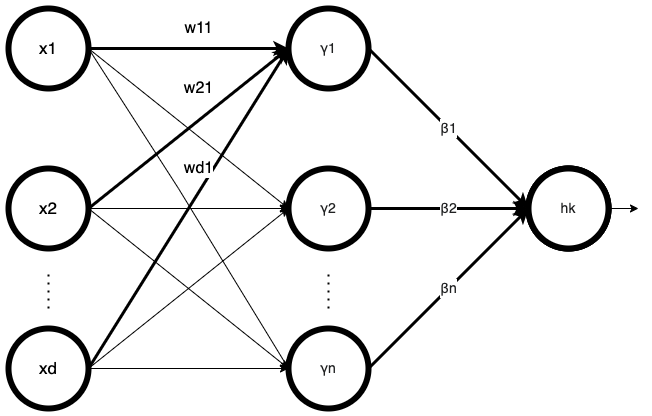
\includegraphics[width=0.65\textwidth]{1-Introduccion_redes_neuronales/Red-Neuronal-una-capa-simple.png}
        \caption{\textit{Grafo} de una red neuronal de una capa oculta}
        \label{img:grafo-red-neuronal-una-capa-oculta_repeticion}
    \end{figure}

\end{frame}

\begin{frame}{Comparativa de definiciniciones de red neuronal}
    Nuestra propuesta: 
    \begin{align*}
                h_k(x) = 
                %\textcolor{teal}{\underline{\hspace{0.4cm}}}
                \sum_{i=1}^{n} \textcolor{teal}{\beta_{i k}} \gamma_{i}( A_{i}(x))
    \end{align*}
    Modelo usual \cite{MostafaLearningFromData}:
    \begin{align*}
        y_k(x) &= 
        \textcolor{red}{\theta_k}
        \left( 
            \sum^n_{j=1} \textcolor{red}{A_{k}}
            \left(
                \sigma 
                \left(
                    A^{d}_{j k}
                    \left(
                        x
                    \right)
                \right)
            \right)
        \right)
    \end{align*}
\end{frame}
\subsection{Modelo bien definido}
\begin{frame}{Las redes neuronales son aproximadores universales}
    \begin{block}{Teorema  \textbf{Las redes neuronales son una clase de aproximadores universales}}
        (Hornik, Stinchcombe y White 1989 \cite{HORNIK1989359})
        Una red neuronal con tan solo \textbf{una capa oculta} y con \textbf{una función de activación cualquiera} es capaz de \textbf{aproximar cualquier 
        función Borel medible}  con dominios y codominios de dimensión finita (no necesariamente iguales) y con el nivel de precisión que se desee \textbf{siempre y cuando 
        se utilicen suficientes neuronas}. En este sentido las redes redes neuronales son una clase de aproximadores universales.
    \end{block}
    En resumen: 
    \begin{equation*}
        \mathcal{H}(\R^d,\R^s)  \textit{ es denso en } \mathcal{M}(\R^d,\R^s) 
    \end{equation*}
\end{frame}

\begin{frame}{Aproximador universal a funciones medibles}
    \label{univeral-aproximator}
    \begin{flushright}
        \textit{Capítulo 2 páginas 47-76}
    \end{flushright}
    Relación ser denso en 
    \begin{align*}
        \rrnn 
            \Rightarrow  
        \rrnng 
            \Rightarrow
        \pmcg
            \Rightarrow  
        \fC    
            \Rightarrow 
        L_p
        \Rightarrow 
        \fM .
    \end{align*}
    Salida múltiple: 
    \begin{equation*}
        \mathcal{H}(\R^d,\R^s)  \textit{ es denso en } \mathcal{M}(\R^d,\R^s) 
    \end{equation*}
    \pause
    ¿Esto computable? 
    \begin{align*}
        h_k(x) = 
        %\textcolor{teal}{\underline{\hspace{0.4cm}}}
        \sum_{i=1}^{n} 
        % \textcolor{teal}
        {\beta_{i k}} \gamma_{i}( A_{i}(x))
\end{align*}
    \pause
    \begin{exampleblock}{Teorema}
        El espacio $\mathcal{H}(\Q^d, \Q^s)$ es denso en el espacio $\mathcal{M}(\R^d,\R^s)$. 
    \end{exampleblock}
\end{frame}



%% ¿Cómo podemos encontrar la red neuronal concreta 
\begin{frame}
\frametitle{Aprendizaje} 
\begin{enumerate}
    \item \textbf{¿Cuánto de cerca estamos de la función ideal?}: Error cuadrático medio. 
    \begin{equation*}
        E_{\mathcal{D}}(h) = \frac{1}{N} \sum_{(x,y) \in \mathcal{D}} \sum_{k=1}^s(h_k(x)- y_k)^2. 
    \end{equation*}
    \pause 
   \item  \textbf{Minimizar el error}: Descenso de gradiente. 
    \begin{equation*}
        h_{t+1}  = h_t - \eta \nabla E_{\mathcal{D}}(h_t) \quad \eta \in \R^+.
    \end{equation*}  

\end{enumerate}  
\end{frame}


\begin{frame}{¿Por qué revindicamos un nuevo modelo?}
    \begin{flushright}
        \textit{Capítulo 5 páginas 79-96}
    \end{flushright}
    Nuestra propuesta: 
    \begin{align*}
                h_k(x) = 
                %\textcolor{teal}{\underline{\hspace{0.4cm}}}
                \sum_{i=1}^{n} \textcolor{teal}{\beta_{i k}} \gamma_{i}( A_{i}(x))
    \end{align*}
    Modelo usual:
    \begin{align*}
        y_k(x) &= 
        \textcolor{red}{\theta_k}
        \left( 
            \sum^n_{j=1} \textcolor{red}{A_{k}}
            \left(
                \sigma 
                \left(
                    A^{d}_{j k}
                    \left(
                        x
                    \right)
                \right)
            \right)
        \right)
    \end{align*}
    Solventamos diferencias: 
    \begin{itemize}
        \item Se puede prescindir de $\theta$ (\textit{Demostración en páginas 83-85)}
        \item ¿Se puede prescindir del sesgo? (\textit{Demostración en páginas 81-83})
    \end{itemize}
\end{frame}

\begin{frame}
    \frametitle{Comparativas de mejoras}
    \begin{table}[h]
        \centering
        \resizebox{\textwidth}{!}{
            \begin{tabular}{| c | c | c | c |}
            \hline
            % cabecera 
            Operación 
            & Coste formulación usual 
            & Coste nuestra propuesta  
            & Operaciones reducidas  \\ \hline
            $+$ & $n(d+s)$ & $n(d+s-1)$ & $n$\\
            $\times$ & $n(d+s+2)$ & $n(d+s)$  & $2n$\\
            $\gamma$ & $n$  & $n$  & $0$ \\
            $\mathfrak{I}$  & $2$ & $0$ & $2$ \\
            \hline
            \end{tabular}
        }
        \caption{Comparativas de coste computacional en evaluación entre la implementación usual de una red neuronal y la nuestra}
        \label{tab:comparativas coste red neuronal }
    \end{table}
    Para $n$ el número de neuronas, $d$,$s$ las dimensiones de entrada y salida de las redes neuronales. 
\end{frame}
\begin{frame}
    \frametitle{¿Qué hemos conseguido hasta aquí?}
    \begin{itemize}
        \item Entender qué son, cómo funcionan y porqué las redes neuronales.
        \item Un modelo que reduce el coste computacional de los usuales.
        \item Implementación del modelo y sus métodos en la biblioteca 
        \textit{OptimizedNeuralNetwork.jl}.
    \end{itemize}
    

\end{frame}


\subsection{Método inicialización aprendida}
%% ¿Cómo podemos encontrar la red neuronal concreta 
\begin{frame}
    \frametitle{¿Qué gran problema tiene le método de aprendizaje propuesto?} 
       \textbf{Minimizar el error}: Descenso de gradiente. 
        \begin{equation*}
            h_{t+1}  = h_t - \eta \nabla E_{\mathcal{D}}(h_t).
        \end{equation*} 
        \pause
        ¿Cómo determinar  \textcolor{red}{$h_0$}? 
        ¿aleatorio? ¿transferencia de características?
\end{frame}

\begin{frame}{Método de inicialización aprendida}
    \begin{flushright}
        \textit{Capítulo 7 páginas 111-130}
    \end{flushright}
    Algoritmo: 
    \begin{enumerate}
        \item Se toma $p \in \R^d$  aleatorio. 
        \item Se extrae un subconjunto aleatorio  $\Lambda \subset \mathcal{D}$
        que satisface 
        \begin{equation*}
            p \cdot (x_i-x_j) \neq 0
        \end{equation*}
        para cualquier $x_i,x_j$ distintos que estén en algún par de $\Lambda$.
        \item Se construye de manera recursiva la red neuronal resolviendo esta sistema de ecuaciones: 
        \begin{equation*}
            \left\{ 
                \begin{array}{l}
                    S_{k} =
                        M -  \frac{2 M}{p \cdot (x_k - x_{k-1})}(p \cdot x_{k})
                    \\
                    A_{k i} = \frac{2 M}{p \cdot (x_k - x_{k-1})}
                    p_{i} 
                    \\
                    B_{* k} = y_k - y_{k-1}
                \end{array}
            \right.
        \end{equation*} 
\end{enumerate}
\end{frame}


\begin{frame}{Visualización de cómo actúa el algoritmo }
    
\begin{figure}[H]
    \centering
    \begin{subfigure}[b]{0.475\textwidth}
        \centering
        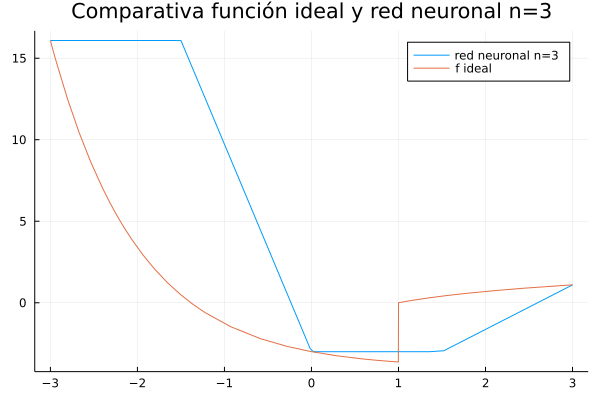
\includegraphics[width=\textwidth]{7-algoritmo-inicializar-pesos/f_ideal_y_rn_con_3_neuronas.png}
    \end{subfigure}
    \hfill
    \begin{subfigure}[b]{0.475\textwidth}  
        \centering 
        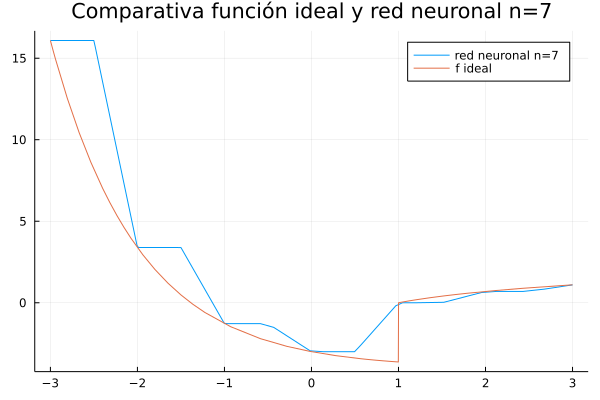
\includegraphics[width=\textwidth]{7-algoritmo-inicializar-pesos/f_ideal_y_rn_con_7_neuronas.png}  
    \end{subfigure}
    \vskip\baselineskip
    \begin{subfigure}[b]{0.475\textwidth}   
        \centering 
        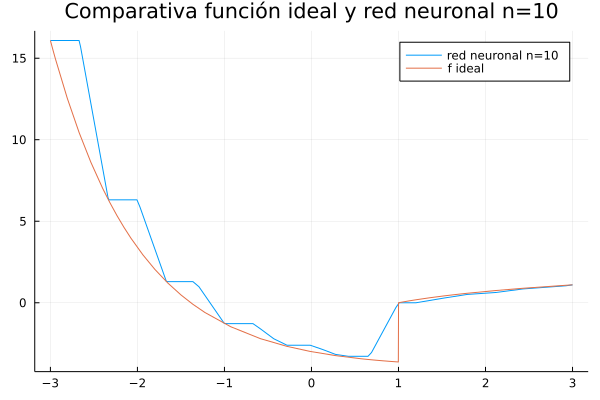
\includegraphics[width=\textwidth]{7-algoritmo-inicializar-pesos/f_ideal_y_rn_con_10_neuronas.png}
    \end{subfigure}
    \hfill
    \begin{subfigure}[b]{0.475\textwidth}   
        \centering 
        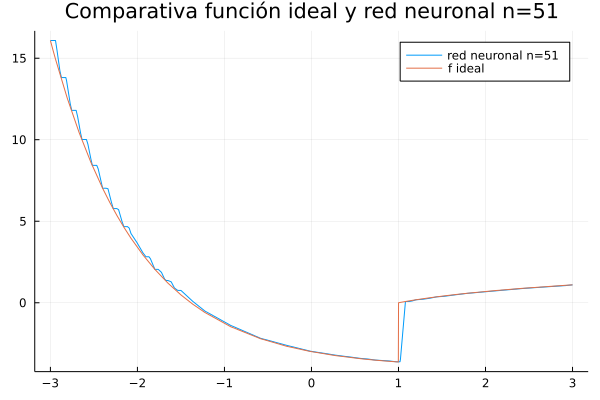
\includegraphics[width=\textwidth]{7-algoritmo-inicializar-pesos/f_ideal_y_rn_con_51_neuronas.png}   
    \end{subfigure}
    \caption{Ejemplo de aproximación de la función $f(x)$ con redes neuronales.} 
    \label{fig:aproximacion-red-neuronal}
\end{figure}
\end{frame}
 

\begin{frame}
    \frametitle{Propuesta de uso del algoritmo de inicialización aprendida}

    \textbf{Diferencias con \textit{backpropagation} filosofía y coste:}
    \begin{itemize}
        \item \textit{Backpropagation}: Fijadas neuronas trato de reducir el error. Coste  $n |\mathcal{D}| >> n^2$.
        \item Algoritmo de inicialización aprendida: A más neuronas menos error. Coste  $n\log(n)$
    \end{itemize}
\textbf{Propuesta de uso}
    \begin{enumerate}
        \item Inicializar red neuronal con nuestro algoritmo de inicialización aprendida. 
        \item Reducir el error con \textit{backpropagation}. 
    \end{enumerate}

\end{frame}

%%%%% Sobre las funciones de activación
\section{Democratización las funciones de activación} 
\begin{frame}
    \frametitle{Democratización de las funciones de activación}
    \begin{flushright}
        \textit{Capítulo 6 páginas 99-109}
    \end{flushright}
    \begin{equation*}
        \sum_{i=1}^{n} \beta_{i k} \textcolor{red}{\gamma_{i}}( A_{i}(x))
    \end{equation*}
    ¿Hay funciones de activación mejores que otras?
\end{frame}
\begin{frame}
    \frametitle{Democratización de las funciones de activación}
    Cambio de enfoque: 

    Ver funciones de activación como curvas en el plano Euclídeo.  

    \begin{exampleblock}{Teorema}
        Sea $\phi \in \mathcal{A}(\R^2)$ una función afín 
        cuya forma matricial asociada es de la forma:  
        \begin{equation*}
            \phi 
            \left( 
                \begin{bmatrix}
                    x & y
                \end{bmatrix}
            \right)
            = 
            \begin{bmatrix}
                x & y
            \end{bmatrix}
            \begin{bmatrix}
                a & 0 \\
                 0& b 
            \end{bmatrix}
            +
            \begin{bmatrix}
                t_x & t_y
            \end{bmatrix}
        \end{equation*}
        con $a,b \in \R^*$ y $t_x, t_y \in \R$.
    
        Sean dos funciones de activación $\sigma, \gamma$ tales que 
        \begin{equation*}
            \phi(Grafo(\sigma)) = Grafo(\gamma),
        \end{equation*}
        entonces 
        el espacio de redes neuronales de $n$ neuronas creado a partir de la función de activación $\sigma$ es  
        igual al espacio de redes neuronales creado a partir la función de activación $\gamma$. 
    \end{exampleblock}
\end{frame}

\begin{frame}
    \frametitle{Se ha minimizado el coste de las funciones de activación de en familias que pueden tener la misma precisión}
    
    \begin{table}[H] 
        \centering  
        \begin{tabular}{| c | c | c | }
            \hline
            \textit{Grupo escalera} & \textit{Grupo sigmoide} & \textit{Grupo ReLU} \\
            \hline
           &  Rampa &  \\
           Indicadora & Sigmoidea & ReLU\\
           Umbral & \textit{Cosine Squasher}& LReLU\\
            & tanh & \\
            & \textbf{\textit{Hard Hyperbolic Function}}& \\
    \hline
        \end{tabular}
        \caption{Propuesta de familia de funciones de activación con mismo potencial}  
        \label{table:Clases-equivalencia-activation-function}
    \end{table}

\end{frame}
\begin{frame}
    \frametitle{Tiempo utilizado en cada iteración}

    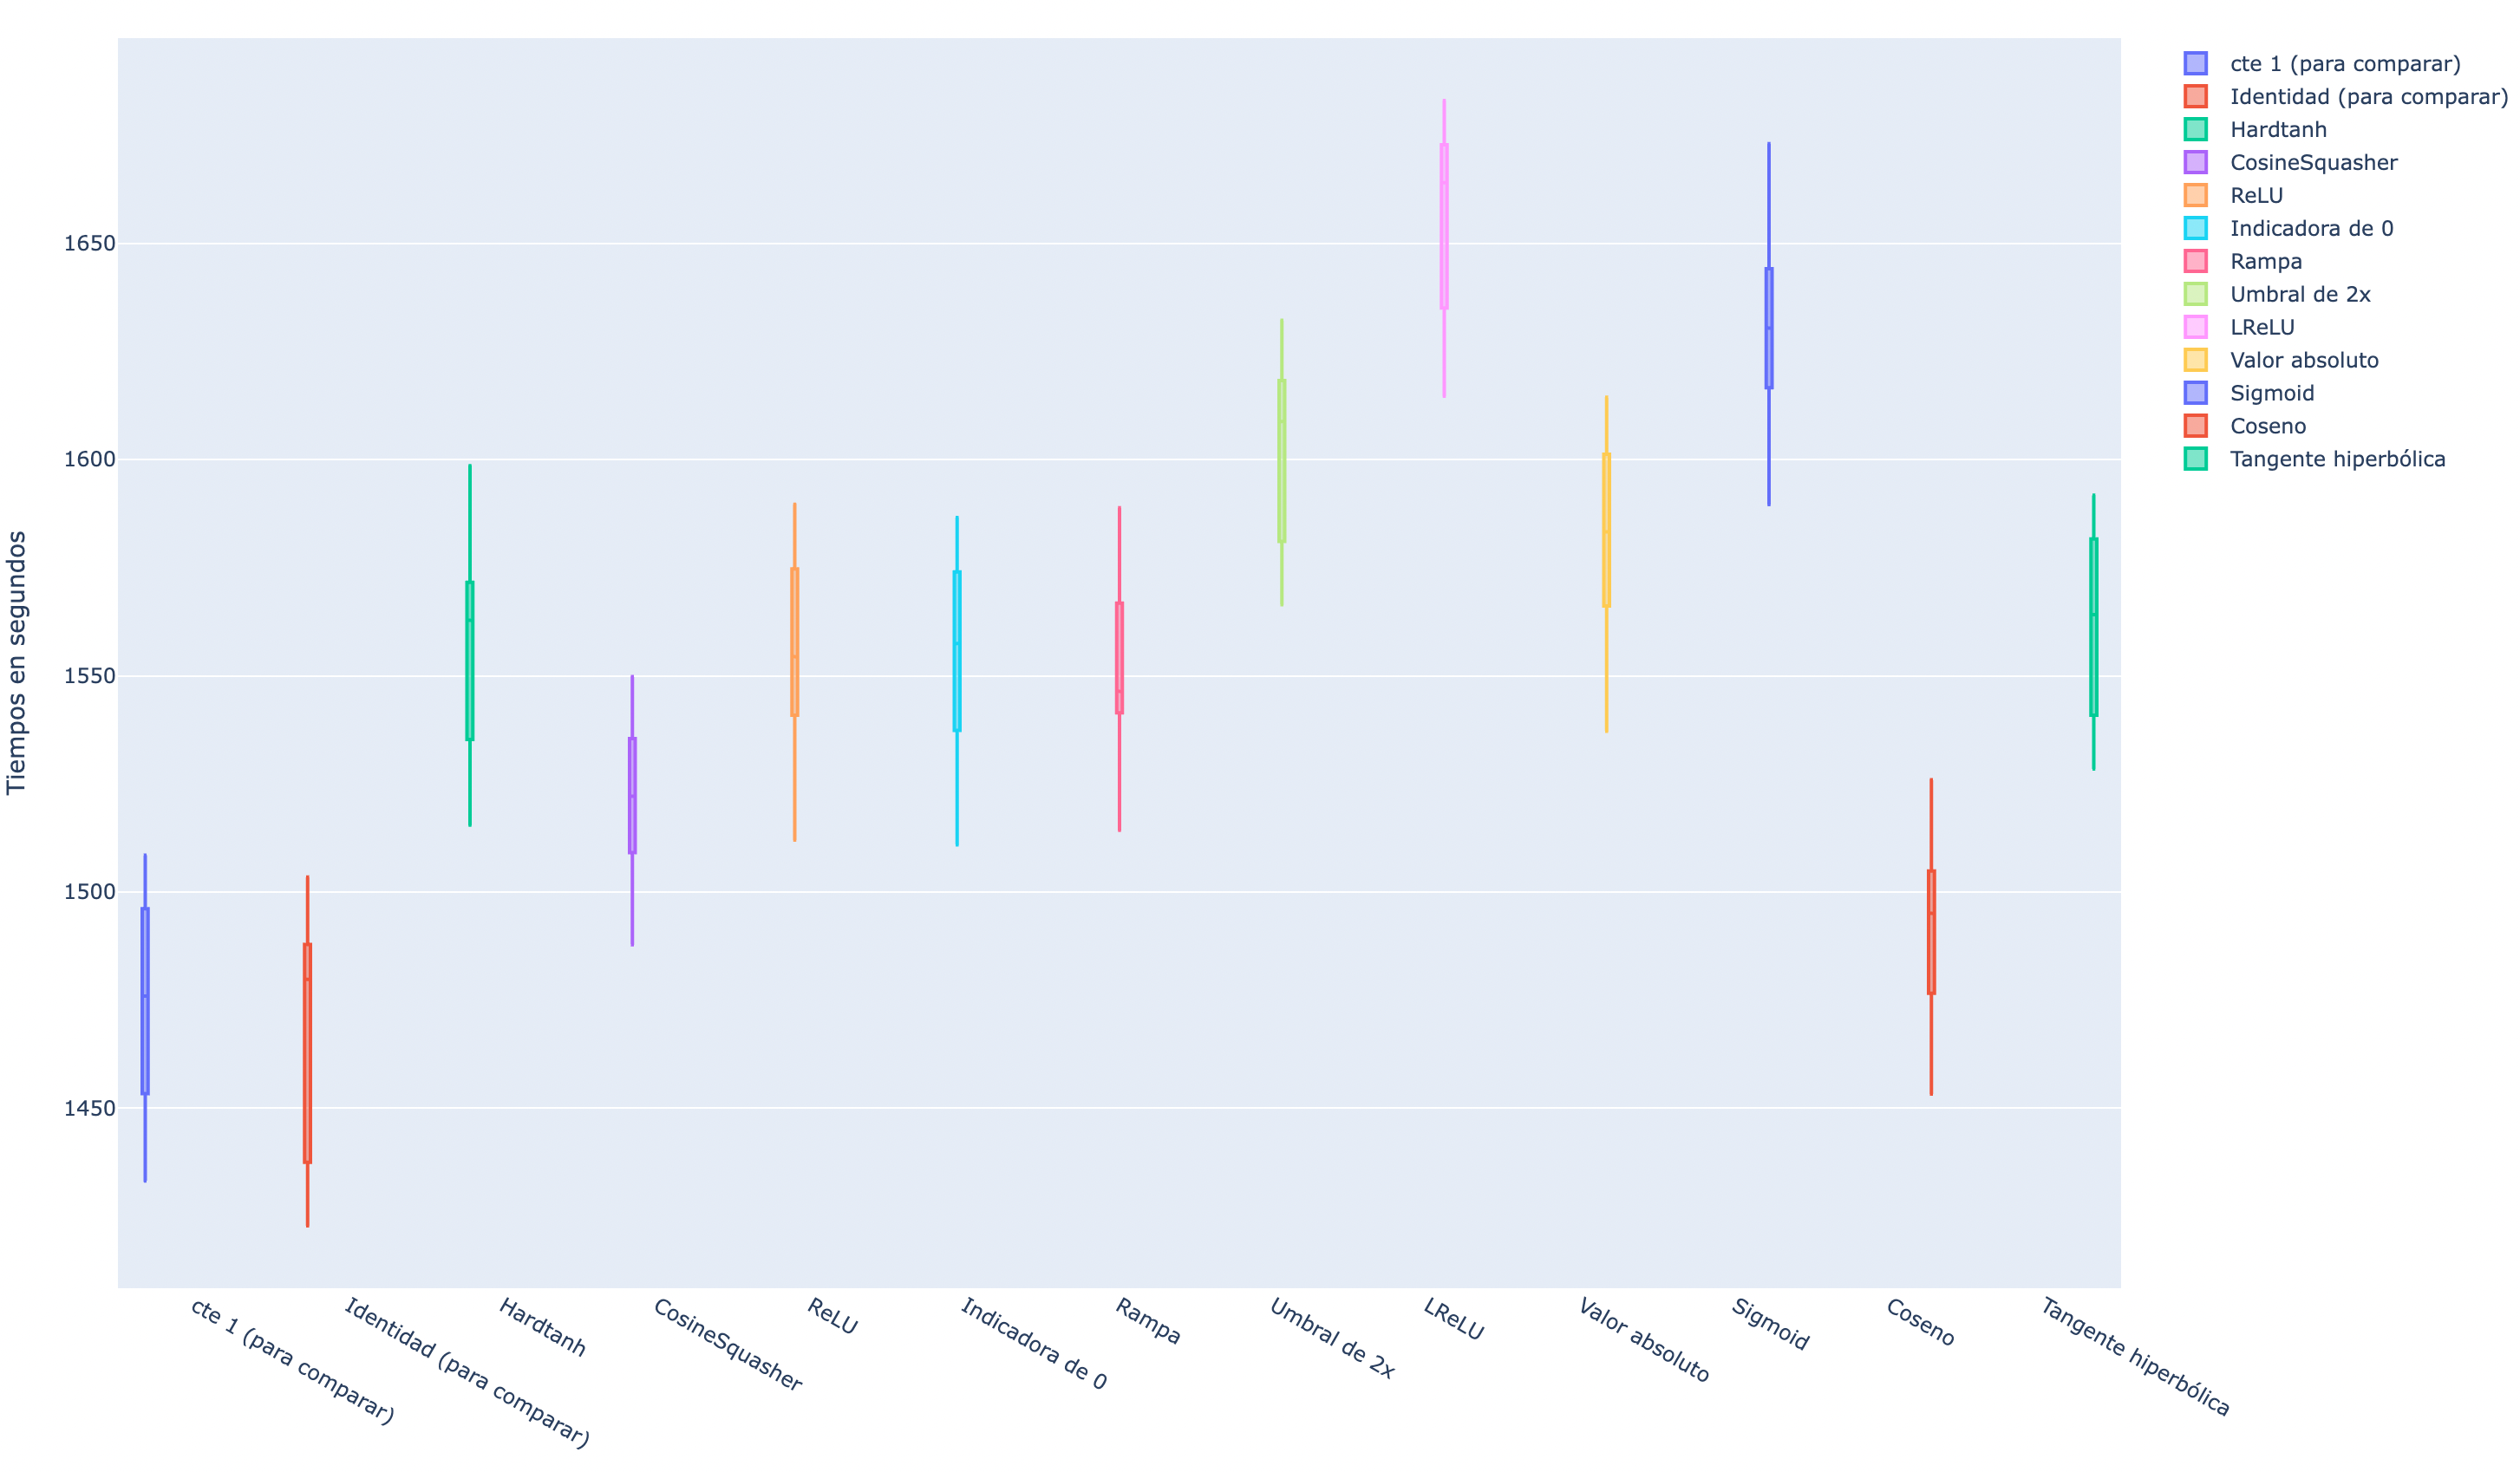
\includegraphics[width=\textwidth]{5-estudio-experimental/activation-function/boxplot-whiskers-activation-function.png}

\end{frame}
\begin{frame}
    \frametitle{Conclusiones}
    \begin{enumerate}
        \item Se ha propuesto y revindicado un nuevo modelo de red neuronal.
        \item Se construido la biblioteca de \textit{OptimizedNeuronalNetwork.jl} que contiene: 
        \begin{itemize}
            \item Modelo propuesto. 
            \item Evaluación.
            \item Aprendizaje. 
            \item Método de inicialización aprendida. 
        \end{itemize}
        \item Se ha propuesto un nuevo método de inicialización de pesos de una red neuronal. 
        \item Se ha propuesto un criterio de inicialización de pesos. 
    \end{enumerate}
    
\end{frame}

%%%% 
%%% bibliografía
\begin{frame}
    \frametitle{Bibliografía}
    \printbibliography
    
\end{frame}

%%%%%%%%%%%%%%%%%%%%%%%%%%%%%%%%%%%%%%%%%%%%%%%%
\section*{Diapositivas a posibles preguntas}

\begin{frame}{Posibles preguntas}
    \begin{itemize}
        \item Aproximador universal espacios intermedios: diapositiva \ref{univeral-aproximator}.
        \item Algunas definiciones: diapositiva \ref{definiciones-esenciales}.
    \end{itemize}
    
\end{frame}
\begin{frame}{Aproximador universal a funciones medibles}
    \label{definiciones-esenciales}
    \begin{align*} 
        \sum \prod^d(G) = \{ 
        &f: \R^r \longrightarrow \R / \quad
        f(x) = \sum_{j = 1} ^q  \beta_j \prod_{k=1}^{l_j}
        G(A_{jk}(x)), \\
        &x  \in \R^d, \beta_j \in \R, A_{jk}\in \afines; l_j,q \in \N
        \}.
    \end{align*} 
    Una función  $\psi: \R \longrightarrow [0,1]$ 
    es una \textbf{ función de activación} 
    si  cumple las siguientes propiedades:
    \begin{itemize}
        \item Es no decreciente.
        \item $\lim _{x \rightarrow \infty} \psi(x) = 1$.
        \item $\lim _{x \rightarrow -\infty} \psi(x) = 0$.
    \end{itemize}   
\end{frame}


\begin{frame}
    \frametitle{Ejemplo con datos reales de resultados del algoritmo de aprendizaje aprendido}
    Ejemplo real con datos \textit{Airfoil Self-Noise} de la NASA: 
    \begin{itemize}
        \item Error medio en test partiendo de red neuronal aleatoria y entrenando con \textit{backpropagation} hasta encontrar mínimo: $0,567 \pm 0,009$.
        \item Error medio en test alcanzado de nuestro algoritmo de inicialización aprendida: $0,171 \pm 0,022$.
    \end{itemize}
\end{frame}


% Para las citas que no estén mencionadas 
\begin{frame}
    \frametitle{Citas no mencionadas en ningún sitio}

    Este cándida diapositiva está solo para que pueda citar la 
    bibliografía y aparezca en la presentación. 
    \cite{MostafaLearningFromData}
    \cite{the-elements-of-real-analysis}

\end{frame}

\end{document}

